\documentclass[]{article}
\usepackage{lmodern}
\usepackage{amssymb,amsmath}
\usepackage{ifxetex,ifluatex}
\usepackage{fixltx2e} % provides \textsubscript
\ifnum 0\ifxetex 1\fi\ifluatex 1\fi=0 % if pdftex
  \usepackage[T1]{fontenc}
  \usepackage[utf8]{inputenc}
\else % if luatex or xelatex
  \ifxetex
    \usepackage{mathspec}
  \else
    \usepackage{fontspec}
  \fi
  \defaultfontfeatures{Ligatures=TeX,Scale=MatchLowercase}
\fi
% use upquote if available, for straight quotes in verbatim environments
\IfFileExists{upquote.sty}{\usepackage{upquote}}{}
% use microtype if available
\IfFileExists{microtype.sty}{%
\usepackage{microtype}
\UseMicrotypeSet[protrusion]{basicmath} % disable protrusion for tt fonts
}{}
\usepackage[margin=1in]{geometry}
\usepackage{hyperref}
\hypersetup{unicode=true,
            pdftitle={Assessment 09 - Data Visualization Principles Part 1},
            pdfauthor={Gabriele Mineo - Harvard Data Science Professional},
            pdfborder={0 0 0},
            breaklinks=true}
\urlstyle{same}  % don't use monospace font for urls
\usepackage{graphicx,grffile}
\makeatletter
\def\maxwidth{\ifdim\Gin@nat@width>\linewidth\linewidth\else\Gin@nat@width\fi}
\def\maxheight{\ifdim\Gin@nat@height>\textheight\textheight\else\Gin@nat@height\fi}
\makeatother
% Scale images if necessary, so that they will not overflow the page
% margins by default, and it is still possible to overwrite the defaults
% using explicit options in \includegraphics[width, height, ...]{}
\setkeys{Gin}{width=\maxwidth,height=\maxheight,keepaspectratio}
\IfFileExists{parskip.sty}{%
\usepackage{parskip}
}{% else
\setlength{\parindent}{0pt}
\setlength{\parskip}{6pt plus 2pt minus 1pt}
}
\setlength{\emergencystretch}{3em}  % prevent overfull lines
\providecommand{\tightlist}{%
  \setlength{\itemsep}{0pt}\setlength{\parskip}{0pt}}
\setcounter{secnumdepth}{0}
% Redefines (sub)paragraphs to behave more like sections
\ifx\paragraph\undefined\else
\let\oldparagraph\paragraph
\renewcommand{\paragraph}[1]{\oldparagraph{#1}\mbox{}}
\fi
\ifx\subparagraph\undefined\else
\let\oldsubparagraph\subparagraph
\renewcommand{\subparagraph}[1]{\oldsubparagraph{#1}\mbox{}}
\fi

%%% Use protect on footnotes to avoid problems with footnotes in titles
\let\rmarkdownfootnote\footnote%
\def\footnote{\protect\rmarkdownfootnote}

%%% Change title format to be more compact
\usepackage{titling}

% Create subtitle command for use in maketitle
\newcommand{\subtitle}[1]{
  \posttitle{
    \begin{center}\large#1\end{center}
    }
}

\setlength{\droptitle}{-2em}

  \title{Assessment 09 - Data Visualization Principles Part 1}
    \pretitle{\vspace{\droptitle}\centering\huge}
  \posttitle{\par}
    \author{Gabriele Mineo - Harvard Data Science Professional}
    \preauthor{\centering\large\emph}
  \postauthor{\par}
    \date{}
    \predate{}\postdate{}
  

\begin{document}
\maketitle

\paragraph{\texorpdfstring{\textbf{Customizing plots - Pie
charts}}{Customizing plots - Pie charts}}\label{customizing-plots---pie-charts}

Pie charts are appropriate:

\textbf{Instructions}

Possible Answers

\begin{itemize}
\tightlist
\item
  When we want to display percentages.
\item
  When ggplot2 is not available.
\item
  When I am in a bakery.
\item
  Never. Barplots and tables are always better. {[}X{]}
\end{itemize}

\paragraph{\texorpdfstring{\textbf{Customizing plots - What's
wrong?}}{Customizing plots - What's wrong?}}\label{customizing-plots---whats-wrong}

What is the problem with this plot?

\begin{figure}
\centering
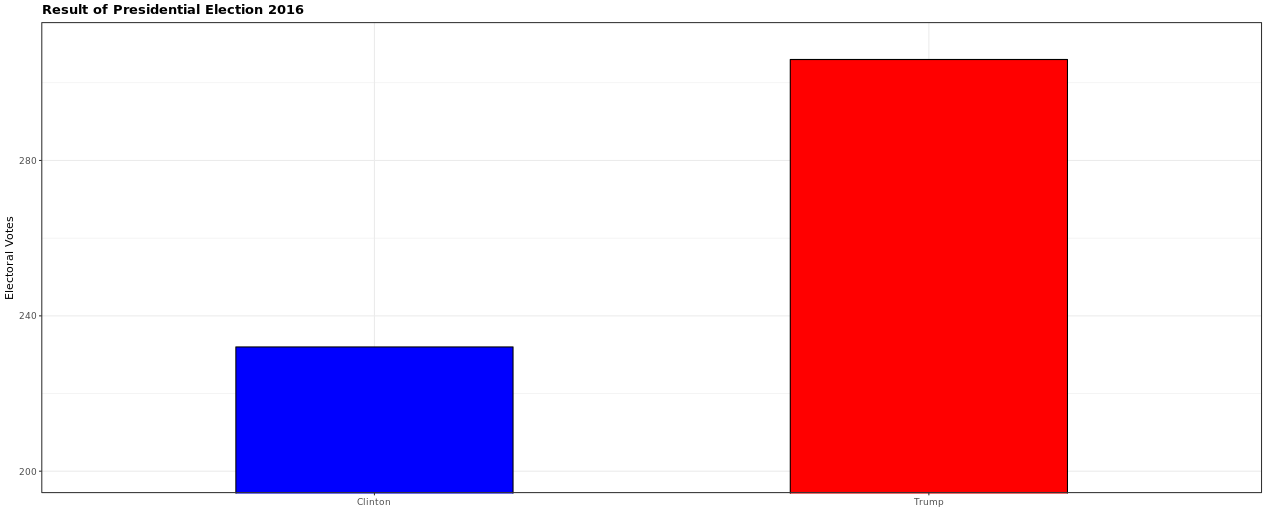
\includegraphics{ex-2.png}
\caption{}
\end{figure}

\textbf{Instructions}

Possible Answers

\begin{itemize}
\tightlist
\item
  The values are wrong. The final vote was 306 to 232.
\item
  The axis does not start at 0. Judging by the length, it appears Trump
  received 3 times as many votes when in fact it was about 30\% more.
  {[}X{]}
\item
  The colors should be the same.
\item
  Percentages should be shown as a pie chart.
\end{itemize}

\paragraph{\texorpdfstring{\textbf{Customizing plots - What's wrong
2?.}}{Customizing plots - What's wrong 2?.}}\label{customizing-plots---whats-wrong-2.}

Take a look at the following two plots. They show the same information:
rates of measles by state in the United States for 1928.

\begin{figure}
\centering
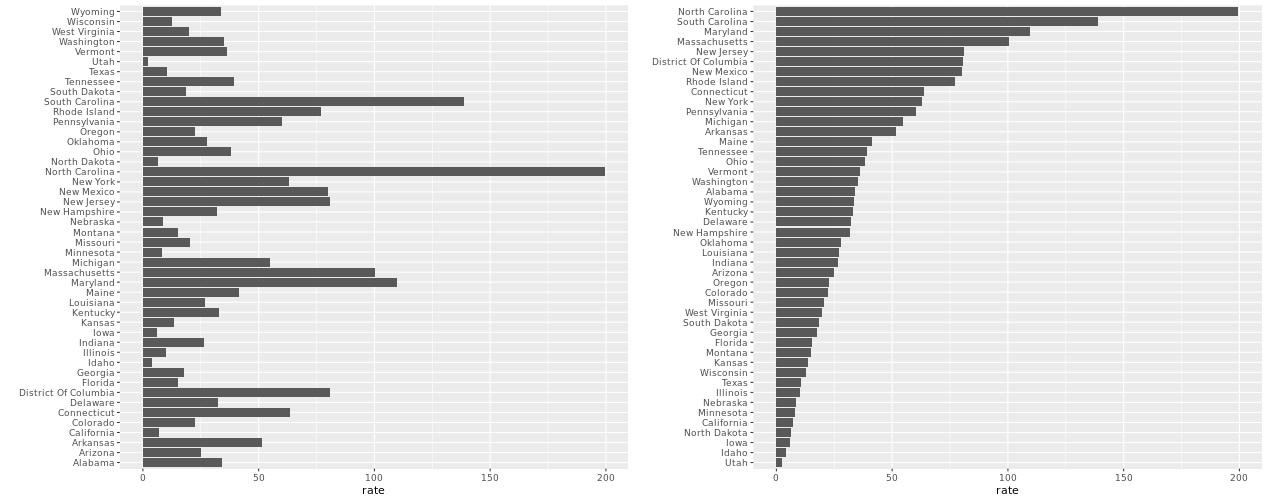
\includegraphics{ex-3.png}
\caption{}
\end{figure}

\textbf{Instructions}

Possible Answers

\begin{itemize}
\tightlist
\item
  Both plots provide the same information, so they are equally good.
\item
  The plot on the left is better because it orders the states
  alphabetically.
\item
  The plot on the right is better because it orders the states by
  disease rate so we can quickly see the states with highest and lowest
  rates. {[}X{]}
\item
  Both plots should be pie charts instead.
\end{itemize}


\end{document}
